% !TEX root = paper.tex
% !TEX encoding = UTF-8 Unicode
% -*- coding: UTF-8; -*-
% vim: set fenc=utf-8
% !TEX spellcheck = en-US
\section{Results}
\label{sec:results}



%------------------------------%
%: see Figure~\ref{fig:results}
\begin{figure}%[!ht]%%[p!]
\centering{(A) \hspace{2.2cm} (B) \hspace{2cm} (C) \hspace{4.6cm} (D)\hspace{1.1cm}}
\centering{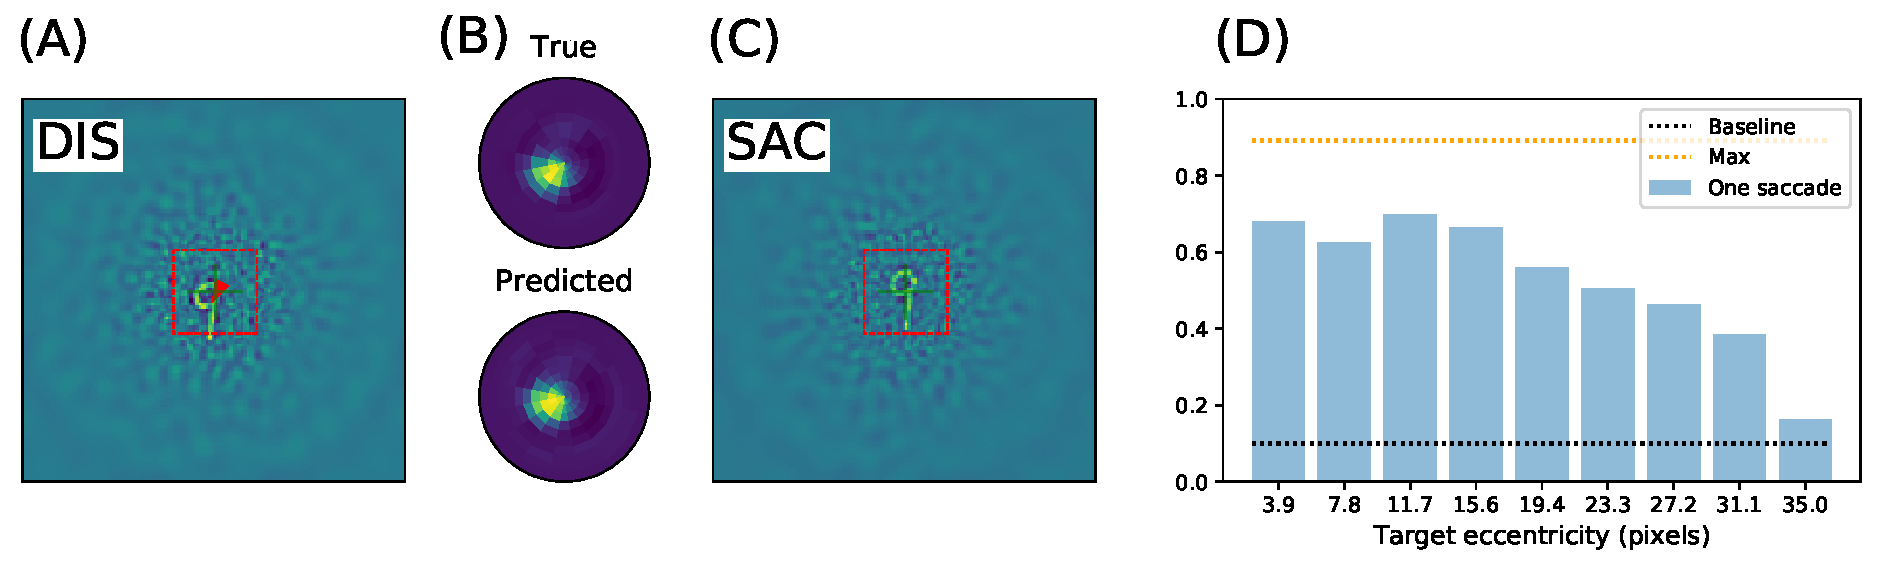
\includegraphics[width=\linewidth]{fig_result}}
\caption{
{\bf Simulated active vision agent results}: 
(A)~The visual display ('DIS', see  Figure~\ref{fig:results}-C)  is transformed into a retinotopic representation which is used as the input to a multi-layer neural network, that transforms the retinal image into an accuracy map. A typical network output after training ('predicted') is compared in (B) with the ground truth ('True'). The network output allows to (C)~generate a saccade to the most likely position in visual space, allowing to estimate a final classification rate. (D)~Testing over a range of 10,000 different trials (different positions and digits), the final average classification accuracy is shown as a function of the eccentricity.
\label{fig:results}}%
\end{figure}%
%%------------------------------%
%result

To test the efficiency of our action selection setup, we estimate the final accuracy as a function of the target eccentricity.

This shows first the results of the 'What' pathway ('No saccade') which quickly drops to baseline level after 3 scales. Second, we show the accuracy results obtained after one saccade which now drops to 'baseline' after 7 scales. This shows that by performing only one saccade, the image is now partly covered.

% energy consumption


% inhibition of return
A particular property of our agent is that at the time when the initial input is presented, two independent inferences are implemented. First, a classification is performed by the 'what' pathway which gives potentially the identity of the digit. Second, an accuracy map is predicted by the 'Where' pathway. It is therefore possible to compare the two maps to chose the most appropriate action: either the  accuracy is best in the 'what' pathway and in that case no saccade is produced. In the other case, a and knowing the accuracy predicted by the what pathway, one can update the accuracy map of the 'where' pathway. Indeed, one knows in particular the accuracy of the 'what' pathway when imposing small shifts to the input. This allows in particular to ``explain away" the current position of the fixation and those which are neighboring (see line 'No saccade' in figure~\ref{fig:results}). Such heuristic gives a principled formulation of the inhibition of return mechanism which is an important aspect for modeling saccades~\citep{Itti01}. In particular, we predict that such a mechanism is dependent on the class of inputs, and would be different for searching for faces as compared to digits.
